% IEEE Transactions on Reliability -- submission draft
% Build: pdflatex manuscript && pdflatex manuscript   (IEEEtran.cls required; bibliography is inline)
\documentclass[journal]{IEEEtran}

\usepackage{amsmath,amssymb,amsthm}
\usepackage{graphicx}
\usepackage{booktabs}
\usepackage{array}
\usepackage{cite}
\usepackage{textcomp}

\newtheorem{proposition}{Proposition}
\newtheorem{assumption}{Assumption}
\newcommand{\E}{\mathbb{E}}
\newcommand{\eps}{\varepsilon}

\begin{document}

\title{Condition-Based Maintenance of Large Language Models\\ Under Knowledge Drift and Imperfect Repair}

\author{Ook Lee%
\thanks{Manuscript received XX XX, 2026; revised XX XX, 2026. (\emph{Corresponding author: Ook Lee.})}%
\thanks{The author is with the Department of Information Systems, Hanyang University, Seoul 04763, Republic of Korea (e-mail: ooklee@hanyang.ac.kr).}}

\markboth{IEEE TRANSACTIONS ON RELIABILITY}%
{Lee: Condition-Based Maintenance of Large Language Models}

\maketitle

\begin{abstract}
A deployed large language model (LLM) is a deteriorating system. Its task-relevant accuracy decays as the world drifts away from the training distribution, and every parameter update risks damaging competence that users already rely on. We cast the resulting decision, namely when to update, by which mechanism, and whether to add an external retrieval store, as a condition-based maintenance problem. Staleness is modeled as a shock-and-wear process driven by a marked point process of drift events, and forgetting as an imperfect repair whose damage is a Fisher-information-weighted quadratic form. For a single-threshold full-retraining policy, a renewal-reward argument gives a square-root law that links update cost, drift intensity, and the optimal cycle length; the same argument shows that a repair leaving less residual damage should be applied more often, not less. For a graduated repair menu, we show that an average-cost Markov decision process admits a nested control-limit policy under stochastic monotonicity and submodularity conditions. Retrieval enters as a compensator that lowers the observed drift rate without repairing the parameters, and a closed-form condition states when the store pays for its upkeep. A measurement study on a public 70-million-parameter model, replicated over ten seeds, supports affine staleness growth, a retrieval-absorbed share equal to corpus coverage, and a mechanism ranking in which an unreplayed low-rank adapter is dominated by taking no action.
\end{abstract}

\begin{IEEEkeywords}
Condition-based maintenance, imperfect maintenance, large language models, Markov decision process, renewal reward, shock-and-wear degradation.
\end{IEEEkeywords}

\section*{Acronyms}
\noindent CBM: condition-based maintenance. LLM: large language model. MDP: Markov decision process. RAG: retrieval-augmented generation. LoRA: low-rank adaptation. EWC: elastic weight consolidation. OLS: ordinary least squares.

\section{Introduction}
\IEEEPARstart{O}{nce} training ends, a large language model begins to age. Facts are superseded, norms shift, and the mix of tasks that users submit moves away from the snapshot on which the parameters were fitted. Organizations respond with a recurring operational decision: whether to retrain or fine-tune, how large a parameter displacement to buy, which update mechanism to use, and whether to keep an independently refreshed retrieval corpus next to the parametric model. In practice this decision is still made by calendar, by incident, or by informal judgment.

The cost structure of the decision is, however, a familiar one. Drift raises an operating-loss rate. Each intervention carries a direct cost that scales with model size and data volume. And unlike a part replacement that returns a machine to a known state, a gradient update can damage competence the organization has already certified. Reliability engineering has a mature vocabulary for exactly this situation: a degradation index, a menu of imperfect repairs, a control-limit policy, and a long-run average-cost criterion \cite{wang2002,jardine2006,vannoortwijk2009,pham1996}. This paper transfers that vocabulary to deployed language models and derives the qualitative shape of the optimal policy.

The transfer is not merely a relabeling. Three features of LLM upkeep have no exact counterpart in classical equipment maintenance, and each has to be modeled explicitly. First, the degradation shock is an external drift event whose magnitude is a mark on a point process, not a physical wear increment. Second, the damage inflicted by a repair is anisotropic in parameter space: moving along directions of high Fisher information on the pre-update task is far more costly, in forgotten accuracy, than moving along unused directions. Third, retrieval-augmented generation supplies a compensator that lowers observed staleness without touching the plant, and therefore without incurring the imperfect-repair penalty.

\subsection{Research Questions}
We address three questions that follow the usual decomposition of a CBM program.
\begin{enumerate}
\item How should the decay of task-relevant accuracy be represented as a function of calendar time and of the unobserved intensity of world change, in a form that can be estimated from a monitoring sample?
\item Given a decision to update, how should the trade-off between absorbing new information and retaining old competence be written so that the organization's tolerance for forgetting becomes an explicit constraint instead of a hidden regularization hyperparameter?
\item What is the long-run cost-minimizing policy over a graduated menu of update mechanisms, and when does an external retrieval store substitute for parametric repair?
\end{enumerate}

\subsection{Contributions}
The paper makes four contributions to the maintenance literature and one measurement contribution.
\begin{enumerate}
\item \emph{Staleness as shock-and-wear.} Knowledge staleness is written as a deterministic leak between events plus jumps at the epochs of a marked point process, in the sense of \cite{vannoortwijk2009}. Under Poisson arrivals the mean path is affine, which recovers the linear degradation curves implicit in empirical retraining-cadence studies as a special case and gives an OLS estimator of the effective drift rate.
\item \emph{Fisher-weighted imperfect repair.} The forgetting penalty used in EWC and related methods \cite{kirkpatrick2017} is recast as an imperfect-repair map. Residual damage after a repair is a scalar that restarts the degradation index above zero, as in the imperfect-maintenance models surveyed in \cite{pham1996}. A direct consequence, not available from the classical replacement model, is that a cheaper and safer repair should be used more often.
\item \emph{Multi-action control limits.} The joint timing-and-mechanism problem is an average-cost MDP on a discretized degradation index crossed with a drift-hazard regime. Under stochastic monotonicity of the transition tails, a total order on the actions, and submodularity of the continuation value, the optimal policy is a nested control-limit rule (Proposition~\ref{prop:cl}). This is the multi-action analogue of the single-threshold policies that are optimal for monotone degradation \cite{barlow1965,wang2002}.
\item \emph{Retrieval as a compensator.} Retrieval lowers the effective drift rate by the share of shocks the corpus can absorb and does not displace parameters. Substituting the reduced rate into the renewal-reward program gives a closed-form investment test: the store is worth its upkeep exactly when the upkeep is below the reduction it creates in the optimal parametric-maintenance cost rate.
\item \emph{Measurement.} The model inputs (staleness slope, retrieval-absorbed share, and per-mechanism cost, effectiveness, and forgetting) are instantiated on the public Pythia-70M checkpoint \cite{biderman2023} with a synthetic world of facts absent from pre-training. Over ten seeds, the study confirms affine growth and a retrieval share equal to coverage, and it exhibits a parameter-efficient update that violates the assumed action order and is dominated by no action.
\end{enumerate}
The paper is a contribution to stochastic maintenance modeling, applied to a digital asset whose repair technology is gradient-based. It does not propose a new continual-learning algorithm, and it is not a field study of a production system.

\subsection{Organization}
Section~\ref{sec:related} reviews related work. Section~\ref{sec:model} defines the system, the degradation index, and the cost accounting. Section~\ref{sec:shock} analyzes the shock-and-wear process and the single-threshold renewal program. Section~\ref{sec:imperfect} develops the imperfect-repair map. Section~\ref{sec:mdp} states the MDP and the control-limit result. Section~\ref{sec:rag} treats retrieval. Section~\ref{sec:num} presents numerical results and the measurement study, and Section~\ref{sec:disc} discusses limitations and operational implications before Section~\ref{sec:concl} concludes. The proof of Proposition~\ref{prop:cl} is in the Appendix.

\section{Related Work}\label{sec:related}
\subsection{Maintenance Optimization and Imperfect Repair}
Deciding when to intervene on a deteriorating system is among the oldest problems in operations research. Age and block replacement policies trade a planned intervention against the cost of failure \cite{barlow1965}. Condition-based policies act on an observed degradation index rather than on age alone \cite{jardine2006,wang2002}, and shock-and-wear and gamma-process models supply the stochastic primitive for that index \cite{vannoortwijk2009}. When a repair does not restore the system to as-good-as-new, the cycle restarts from a residual damage level; \cite{pham1996} organizes the resulting imperfect-maintenance family. Broader reviews are given in \cite{dekker1996,dejonge2020}, and \cite{arts2025} reflects on fifty years of the field, stressing the gap between stylized control-limit theory and the logistics of carrying out a repair.

The present model belongs to this lineage. The degradation index is additive staleness plus residual forgetting; the action set is a totally ordered menu of imperfect repairs plus a no-action option; and the criterion is the long-run average cost of operating loss, intervention spend, and one-off regression cost. What is new is the geometry of the imperfect-repair map and the presence of a compensator that does not repair the plant.

\subsection{Retraining Under Concept Drift}
For classical statistical models the analogue of the replacement decision is the retraining trigger. Lu \emph{et al.} \cite{lu2019} distinguish sudden, gradual, incremental, and recurring drift and catalog detection statistics. Two philosophies recur and mirror the age-based versus condition-based dichotomy: periodic retraining on a fixed calendar, and informed retraining triggered by a drift statistic. Mahadevan and Mathioudakis \cite{mahadevan2023} treat timing as a cost-minimization problem on a stream and show that a cost-aware policy dominates naive drift alarms. Beytur \emph{et al.} \cite{beytur2025} study a budget-constrained trainer facing random concept durations and show that the optimal policy depends on the ageing property of the duration law: decreasing and increasing mean residual life prescribe opposite reactions to a long quiet spell. Williams \emph{et al.} \cite{williams2026} give a rare empirical cadence comparison on a clinical prediction model, finding that monthly retraining was non-inferior to weekly retraining at roughly one quarter of the compute. This diminishing-returns pattern is what a square-root optimal interval predicts, as Section~\ref{sec:shock} makes explicit.

These works address when to retrain a cheap classical model. They do not treat a repair that damages the system, they offer no menu of mechanisms with distinct cost--effectiveness--forgetting profiles, and they have no compensator that can be refreshed independently of the parameters.

\subsection{Forgetting, Knowledge Editing, and Retrieval}
Catastrophic forgetting, the overwriting of earlier representations by a sequential update, is the imperfect-repair phenomenon of neural networks \cite{kirkpatrick2017,shi2024,luo2023}. EWC approximates the pre-update posterior by a Gaussian whose precision is a Fisher information matrix and adds the corresponding quadratic penalty to the next-task loss; later work has criticized the multi-task recursion and the empirical-Fisher surrogate \cite{huszar2018,kunstner2019}. We do not propose a better regularizer. We treat the quadratic form as the organization's constraint set, so that the amount of forgetting purchased by an update becomes an auditable scalar in the maintenance cost instead of a tuning knob inside a trainer.

Knowledge editing aims to rewrite a narrow fact while leaving unrelated behavior untouched \cite{wang2024,zhang2024}, and parameter-efficient fine-tuning such as LoRA \cite{hu2022} restricts the displacement to a low-rank or sparse subspace. In maintenance terms, both correspond to repairs that touch a small subset of components. Retrieval-augmented generation \cite{gao2023} differs in kind: the corpus is updated continuously and generation is conditioned on retrieved passages, so observed staleness can fall without any parameter displacement. Section~\ref{sec:rag} reads this architecture as a compensator in the control-theoretic sense.

\subsection{Cost Structure}
Kaplan \emph{et al.} \cite{kaplan2020} and Hoffmann \emph{et al.} \cite{hoffmann2022} document power-law training cost in model size, data size, and compute. A forward pass costs about two floating-point operations per parameter per token, and the backward pass adds a similar amount for each parameter on the path, so full retraining scales as six operations per parameter per token. Parameter-efficient mechanisms shrink the trainable subset but still pay a forward pass through the whole network, so their cost advantage is smaller than the trainable-parameter count suggests. Alignment updates add a further imperfect-repair channel: reinforcement fine-tuning improves conformity to current preferences at some cost to previously acquired capability, the ``alignment tax'' of \cite{ouyang2022}. In our model that tax is simply a large forgetting increment on a broad update.

\subsection{Gap}
Table~\ref{tab:gap} summarizes the mapping. Continual learning tells the maintainer how to execute an update, concept-drift work tells the maintainer when to trigger a cheap classical model, scaling laws say how costly a given update is, and CBM says how to control a deteriorating physical system. No strand jointly optimizes when, how much, and by which mechanism under a single average-cost criterion that charges both forgetting and money. That joint program is the subject of Sections~\ref{sec:model}--\ref{sec:rag}.

\begin{table}[t]
\caption{Literature Strands and the Questions They Leave Open}\label{tab:gap}
\centering
\footnotesize
\begin{tabular}{p{0.20\columnwidth}p{0.26\columnwidth}p{0.20\columnwidth}p{0.22\columnwidth}}
\toprule
Strand & Representative work & Question answered & Left open\\
\midrule
Continual learning & \cite{kirkpatrick2017,luo2023} & Update without losing competence & When to update; monetary cost\\
Editing and retrieval & \cite{gao2023,wang2024} & Update narrowly, or without touching parameters & Scheduling; joint cost\\
Concept drift / MLOps & \cite{lu2019,mahadevan2023,beytur2025} & When to trigger a cheap model & Expensive, damaging repairs\\
Scaling and alignment & \cite{kaplan2020,ouyang2022} & How costly an update is & Retention and scheduling\\
CBM / imperfect repair & \cite{wang2002,pham1996,dejonge2020} & Optimal maintenance of a deteriorating system & Learned models whose repair damages the plant\\
\bottomrule
\end{tabular}
\end{table}

\section{System Description, Degradation Index, and Costs}\label{sec:model}
\subsection{The Deployed Model}
Let $\theta(t)$ denote the parameter vector of the deployed model at time $t$, with $\theta(0)$ the checkpoint produced by initial training. Between maintenance epochs the vector is held fixed. A maintenance event at time $\tau_k$ replaces $\theta(\tau_k^-)$ by $\theta(\tau_k^+)=\theta(\tau_k^-)+\Delta\theta_k$. A full retrain corresponds to an unconstrained and typically large displacement; a knowledge edit or parameter-efficient fine-tune corresponds to a sparse or low-rank displacement; a retrieval event corresponds to $\Delta\theta_k=0$ together with an update of an external corpus $C(t)$. The world state $W(t)$ is an exogenous stochastic process representing the distribution of facts, tasks, and norms the model will be asked to handle.

\subsection{Freshness, Staleness, and Forgetting}
Task-relevant accuracy, or freshness, is the expected per-example utility of parameters $\theta$ against world $W$,
\begin{equation}
A(\theta,W)=\E_{x\sim W}\big[u(\theta;x)\big],
\end{equation}
where $u$ is bounded (an indicator of correctness, a preference score, or a negative loss). Staleness at time $t$ since the last maintenance epoch $\tau$ is
\begin{equation}
S(t)=A\big(\theta(\tau^+),W(\tau)\big)-A\big(\theta(\tau^+),W(t)\big).
\end{equation}
$S(t)$ is nonnegative in expectation whenever the world drifts away from the post-maintenance snapshot, and $S(\tau^+)=0$ by construction. Because $u$ is bounded, so is $S$; the affine growth models of Section~\ref{sec:shock} are local approximations valid while staleness lies well below that bound.

Forgetting incurred by a displacement $\Delta\theta$ is the drop in accuracy on the pre-update world, with $W$ held fixed:
\begin{equation}
F(\Delta\theta)=A\big(\theta(\tau^-),W(\tau^-)\big)-A\big(\theta(\tau^-)+\Delta\theta,W(\tau^-)\big).
\end{equation}
In reliability terms $F$ is the damage inflicted by an imperfect repair \cite{pham1996}. It depends on the Euclidean size of $\Delta\theta$ and on its alignment with high-curvature directions of the pre-update loss, a dependence made explicit in Section~\ref{sec:imperfect}.

\subsection{Degradation Index}
Staleness and forgetting are measured against different worlds, so neither alone describes the condition of the model after an imperfect update. The degradation index
\begin{equation}
D(t)=S(t)+F(\Delta\theta_{\mathrm{last}})
\end{equation}
starts at $F(\Delta\theta_k)$ immediately after the $k$th maintenance event and then grows as the world drifts. Adding the two terms treats accuracy lost on the old world and accuracy lost to drift as commensurable, which is part of Assumption~\ref{as:scalar}. When a repair induces no forgetting, $D$ coincides with $S$. The index plays the role that a wear or damage process plays in classical CBM.

\subsection{Cost Accounting}
Following the floating-point accounting of the scaling-law literature, an update that trains $n_{\mathrm{train}}$ parameters over $T$ tokens, and whose backpropagation traverses $n_{\mathrm{back}}$ parameters, costs
\begin{equation}
K=\kappa\,T\,(2n_{\mathrm{all}}+2n_{\mathrm{back}}+2n_{\mathrm{train}}),
\end{equation}
where $\kappa$ converts operations to money or opportunity cost and $n_{\mathrm{all}}$ is the full parameter count. Full retraining sets $n_{\mathrm{train}}=n_{\mathrm{back}}=n_{\mathrm{all}}$ and recovers the familiar six-operations rule. Parameter-efficient mechanisms have $n_{\mathrm{train}}\ll n_{\mathrm{all}}$ but still pay the forward pass and a partial backward pass. A simpler trainable-parameter accounting, $K'=6\kappa\,n_{\mathrm{train}}T$, coincides with $K$ for full fine-tuning and understates the cost of efficient mechanisms; it is used in Section~\ref{sec:num} as a lower bound that isolates the part of cost that differs across mechanisms. Retrieval events incur an indexing cost $k_C$ per unit time that scales with corpus size rather than model size.

The long-run objective is to choose maintenance times, displacements, and corpus updates to minimize the average cost rate
\begin{multline}
J=\limsup_{T\to\infty}\frac{1}{T}\,\E\Big[\int_0^T c_L D(t)\,dt\\
+\sum_{\tau_k\le T}\big(K(\Delta\theta_k)+c_F F(\Delta\theta_k)\big)+\int_0^T k_C\,\mathbf 1_{\{C\ \mathrm{active}\}}\,dt\Big].
\end{multline}
Here $c_L$ converts degradation into an operating-loss rate (lost users, compliance exposure, downstream error), and $c_F$ is a one-off charge per unit of forgetting (regression triage, recertification, visible behavioral change). Forgetting is charged twice by design: once as an event cost through $c_F$, and once as a flow cost through $c_L$ for as long as residual damage remains in $D$. Setting $c_F=0$ keeps only the flow cost.

\subsection{Standing Assumptions}
\begin{assumption}[Scalar additive accuracy]\label{as:scalar}
Freshness is a scalar, and staleness and forgetting are commensurable in $D$. In deployment a model is scored on many axes that can drift at different rates; Section~\ref{sec:disc} returns to the vector extension.
\end{assumption}
\begin{assumption}[Exogenous world]\label{as:exo}
$W(t)$ does not depend on the model's own outputs.
\end{assumption}
\begin{assumption}[Discrete maintenance]\label{as:disc}
Actions are events. Continuous adaptation is the limit in which the minimum inter-event time vanishes.
\end{assumption}
\begin{assumption}[Independent marks]\label{as:marks}
Drift magnitudes $\xi_i$ are independent and identically distributed with finite mean $\mu_\xi$, independent of the arrival process.
\end{assumption}
\begin{assumption}[Local optimality]\label{as:local}
Immediately before an update, $\theta$ is approximately a local minimum of the loss on the old world, so that the loss admits a second-order expansion with a diagonal Fisher matrix $I(\theta)$.
\end{assumption}
\begin{assumption}[Monotone MDP structure]\label{as:monotone}
For each drift regime: (i) the tail probabilities of the next degradation state are nondecreasing in the current state for every action; (ii) the action set is totally ordered by nondecreasing effectiveness and nondecreasing cost; (iii) the expected continuation value is submodular in the state--action pair. The chain is unichain.
\end{assumption}

\section{Shock-and-Wear Staleness and the Single-Threshold Program}\label{sec:shock}
\subsection{Drift as a Marked Point Process}
Drift events, the discrete moments at which $W(t)$ shifts enough to be behaviorally consequential, arrive as a marked point process $\{(T_i,\xi_i)\}$, where $T_i$ are epochs and $\xi_i$ are magnitudes satisfying Assumption~\ref{as:marks}. In the Poisson case the arrival rate is $\lambda$. More generally the inter-arrival law $G$ has hazard $h(\cdot)$, which allows drift seasons with increasing or decreasing mean residual life, the distinction emphasized in \cite{beytur2025} and consistent with the taxonomy of \cite{lu2019}.

Between events, staleness accumulates through ordinary exposure to a slowly moving world (vocabulary drift, slow factual turnover), modeled as a deterministic leak $\beta$. At each event it jumps by the mark:
\begin{equation}
dS(t)=\beta\,dt+\sum_i\xi_i\,\delta_{T_i}(dt),\qquad S(\tau^+)=0,
\end{equation}
which is a shock-and-wear equation of the kind used for physical systems \cite{vannoortwijk2009}. Fig.~\ref{fig:path} shows a simulated sample path together with the mean-path approximation used below. By Wald's identity and Assumption~\ref{as:marks},
\begin{equation}
\E[S(t)]=\beta t+\mu_\xi\,m(t),
\end{equation}
where $m(t)$ is the renewal function of the arrival process on an interval of length $t$. In the Poisson case $m(t)=\lambda t$, so expected staleness grows affinely with slope $\gamma:=\beta+\lambda\mu_\xi$. The affine form is a local approximation: in a finite world of facts it saturates once events begin to revisit items that are already stale.

\begin{figure}[t]
\centering
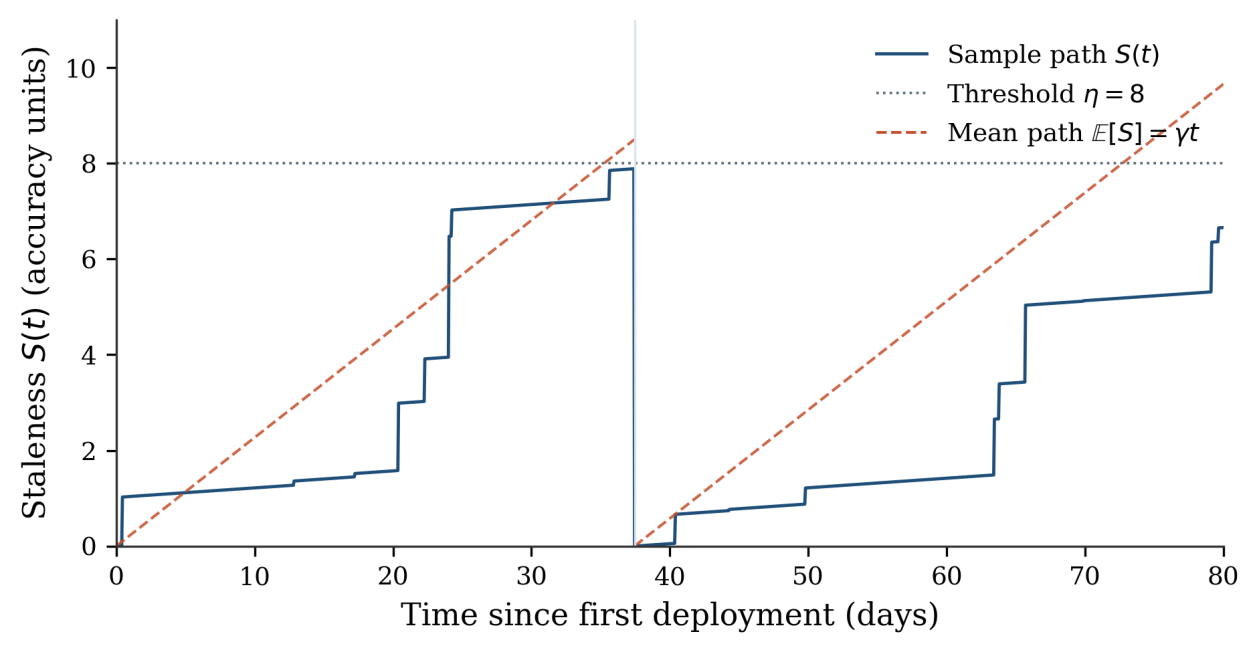
\includegraphics[width=\columnwidth]{figs/fig1_sample_path.png}
\caption{Illustrative shock-and-wear sample path of staleness under a control-limit policy. Jumps are drift events; the dashed line is the mean path on each cycle; the dotted line is the intervention threshold. After each full retrain the index resets to zero.}\label{fig:path}
\end{figure}

\subsection{Renewal-Reward Optimum for Full Retraining}
Consider first the restricted class in which maintenance is always a perfect full retrain ($F=0$, $S(\tau^+)=0$), triggered when expected staleness first reaches a threshold $\eta$. This is a control-limit policy on the degradation index. Under a mean-path approximation the cycle length is $t(\eta)=\eta/\gamma$, which is accurate when individual marks are small relative to $\eta$ so that overshoot is negligible. Let $K_R$ be the retrain cost. The renewal-reward theorem \cite{ross1996} gives the long-run average cost rate
\begin{equation}
J(\eta)=\frac{K_R+c_L\int_0^{t(\eta)}\gamma s\,ds}{t(\eta)}=\frac{K_R\gamma}{\eta}+\frac{c_L\eta}{2}.
\end{equation}
Minimizing over $\eta$ produces the classical square-root form
\begin{equation}
\eta^\ast=\sqrt{\frac{2K_R\gamma}{c_L}},\qquad t^\ast=\sqrt{\frac{2K_R}{c_L\gamma}},\qquad J^\ast=\sqrt{2K_R c_L\gamma}.
\label{eq:sqrt}
\end{equation}
Two comparative-static predictions follow at once and are the simplest testable implications of the model.

\emph{Prediction 1.} The optimal calendar interval $t^\ast$ shrinks with the square root of drift intensity $\gamma$, while the tolerated staleness $\eta^\ast$ grows with the square root of $\gamma$. Faster drift calls for more frequent maintenance in calendar time, but each cycle is allowed to end at a higher staleness level. A fourfold rise in $\gamma$ halves $t^\ast$ and doubles $\eta^\ast$; it does not quarter the interval. Naive ``match the drift rate'' heuristics therefore overreact.

\emph{Prediction 2.} The optimal interval grows only with the square root of the retrain cost. An order-of-magnitude increase in $K_R$, of the kind implied by scaling laws when one moves to a much larger model, lengthens $t^\ast$ by a factor of about three, not ten. Stretching the cadence in proportion to cost leaves expensive models stale for too long. The same curvature is consistent with the clinical finding of \cite{williams2026} that a fourfold reduction in frequency (weekly to monthly) was non-inferior while saving three quarters of the computation.

\subsection{Non-Poisson Arrivals and the Hazard Regime}
When arrivals are not Poisson, $m(t)$ is nonlinear and the conditional intensity over the coming interval depends on the time elapsed since the last event, information that a policy monitoring only $S$ ignores. Maintenance cannot pre-empt a shock that has not occurred; elapsed time matters because it changes the rate at which staleness is expected to accumulate after the next repair and therefore, through the square-root relation, the economically appropriate cycle.

Carrying over the ageing distinction of \cite{beytur2025} gives two hypotheses rather than theorems. Under decreasing mean residual life, a long quiet interval signals that the next shock is expected sooner, which raises the near-term $\gamma$ and shortens the indicated calendar interval. Under increasing mean residual life the opposite adjustment is indicated, and a heuristic that treats every quiet spell as a reason to maintain sooner is miscalibrated. The two regimes can be told apart from the hazard of drift-detector alarms. Section~\ref{sec:mdp} folds the distinction into the MDP as an exogenous regime variable, so that the direction of the threshold shift is a numerical output and not an assumption.

\subsection{Estimating the Decay Parameters}\label{sec:est}
The parameters $\beta$, $\lambda$, and $\mu_\xi$, or more generally $m(\cdot)$, are not observed directly. They can be recovered from a monitoring pipeline that periodically scores the deployed model against held-out, freshly collected evaluation data, which is the infrastructure already recommended in the concept-drift literature. Because $\E[S(t)]$ is affine in $t$ between maintenance events, the slope $\gamma$ is the coefficient of an OLS regression of measured staleness on time since the last repair, pooled across cycles. A nonzero intercept reflects residual error of the freshly maintained model and does not affect the slope. Departures from affinity diagnose either non-Poisson arrivals or saturation. Section~\ref{sec:num} runs this regression on a public model.

\section{Imperfect Repair: Fisher-Constrained Forgetting}\label{sec:imperfect}
\subsection{Forgetting as Displacement Geometry}
Assumption~\ref{as:local} and the Laplace argument underlying EWC give a second-order expansion of the pre-update loss $L_{\mathrm{old}}$ about $\theta(\tau^-)$,
\begin{equation}
L_{\mathrm{old}}(\theta(\tau^-)+\Delta\theta)\approx L_{\mathrm{old}}(\theta(\tau^-))+\tfrac12\,\Delta\theta^{\!\top} I(\theta(\tau^-))\,\Delta\theta,
\end{equation}
where $I$ is the diagonal-approximated Fisher matrix on the old world and the linear term vanishes at a local minimum. Taking accuracy loss as proportional to the rise in loss, with the constant absorbed into the units,
\begin{equation}
F(\Delta\theta)\approx\tfrac12\,\Delta\theta^{\!\top} I(\theta(\tau^-))\,\Delta\theta.
\label{eq:fisher}
\end{equation}
Equation~\eqref{eq:fisher} is the penalty added to the training objective under EWC. The modeling choice here is to treat it as a constraint that enters the maintenance cost, so that the organization's tolerance $\eps$ for forgetting is an explicit, auditable quantity.

\subsection{The Constrained Update}
Given a target staleness reduction $\pi_{\mathrm{target}}$ that the repair is meant to deliver, the update problem at a maintenance epoch is
\begin{equation}
\min_{\Delta\theta}\ K(\Delta\theta)\quad\text{s.t.}\quad \pi(\Delta\theta)\ge\pi_{\mathrm{target}},\ \ F(\Delta\theta)\le\eps.
\end{equation}
By the accounting of Section~\ref{sec:model}, the mechanism-dependent part of $K$ grows with the number of parameters touched and with how deep in the network they lie. The program therefore trades sparsity and locality of the displacement against cost and against the Fisher-weighted norm. This is the formal reason that a knowledge edit confined to a small subspace can purchase plasticity at negligible stability cost. It is also the reason that ``parameter-efficient'' is not synonymous with ``low forgetting'': a low-rank adapter bounds the Euclidean size of $\Delta\theta$, not its Fisher-weighted size. Section~\ref{sec:num} records a measured violation.

\subsection{Stability--Plasticity Frontier}
Plasticity is the staleness reduction delivered by $\Delta\theta$; stability cost is $F(\Delta\theta)$. For a fixed budget $K$, the Pareto frontier of this bi-objective problem is governed by the alignment between the gradient that reduces staleness on new data and the leading eigenvectors of $I$. When those directions are nearly orthogonal, the regime that knowledge editing is designed to exploit, the frontier is flat and large plasticity can be bought cheaply in forgetting. When they are nearly parallel, as in a broad alignment update, the frontier is steep and every unit of new-behavior plasticity is bought at substantial cost to old-behavior stability. Mixing the new objective with the original pre-training loss, the mitigation used in \cite{ouyang2022}, is a device for biasing $\Delta\theta$ toward directions with a smaller $I$-weighted norm.

\subsection{Imperfect Repair Inside the Renewal Program}
A nonzero forgetting event leaves residual damage $F$ at the moment of maintenance, so $D$ restarts at $F$ rather than at zero. Consider a policy that applies the same mechanism whenever $D$ reaches $\eta$. Under the mean-path approximation, a cycle lasts $(\eta-F)/\gamma$ and the integrated degradation over the cycle is $(\eta+F)(\eta-F)/(2\gamma)$. Charging $c_F F$ once per cycle yields
\begin{equation}
J(\eta;F)=\frac{(K+c_F F)\,\gamma}{\eta-F}+\frac{c_L(\eta+F)}{2}.
\end{equation}
Writing $\eta=F+\delta$ and minimizing in $\delta$ gives
\begin{equation}
\delta^\ast=\sqrt{\frac{2(K+c_F F)\gamma}{c_L}},\quad t^\ast=\frac{\delta^\ast}{\gamma},\quad J^\ast=\sqrt{2c_L\gamma\,(K+c_F F)}+c_L F.
\end{equation}
The optimal cost rate therefore rises through two channels: the effective one-off cost inflates from $K$ to $K+c_F F$, and a permanent flow $c_L F$ remains that no cadence can remove. Holding $K$ fixed, a mechanism with smaller $F$ has a smaller effective one-off cost and therefore a smaller $\delta^\ast$ and a shorter optimal interval. \emph{Safer repairs should be used more often, not less.} When mechanisms differ in both $K$ and $F$ they must be compared through the minimized $J^\ast$, not through $K$ or $F$ alone: a cheap mechanism with large residual damage can lose to an expensive perfect repair because of the permanent term. This comparative static runs opposite to the drift-intensity effect in Section~\ref{sec:shock} and is the second closed-form prediction of the paper. Fig.~\ref{fig:cost} shows the resulting U-shaped cost-rate curves and the rightward shift of the minimizer as residual damage grows.

\begin{figure}[t]
\centering
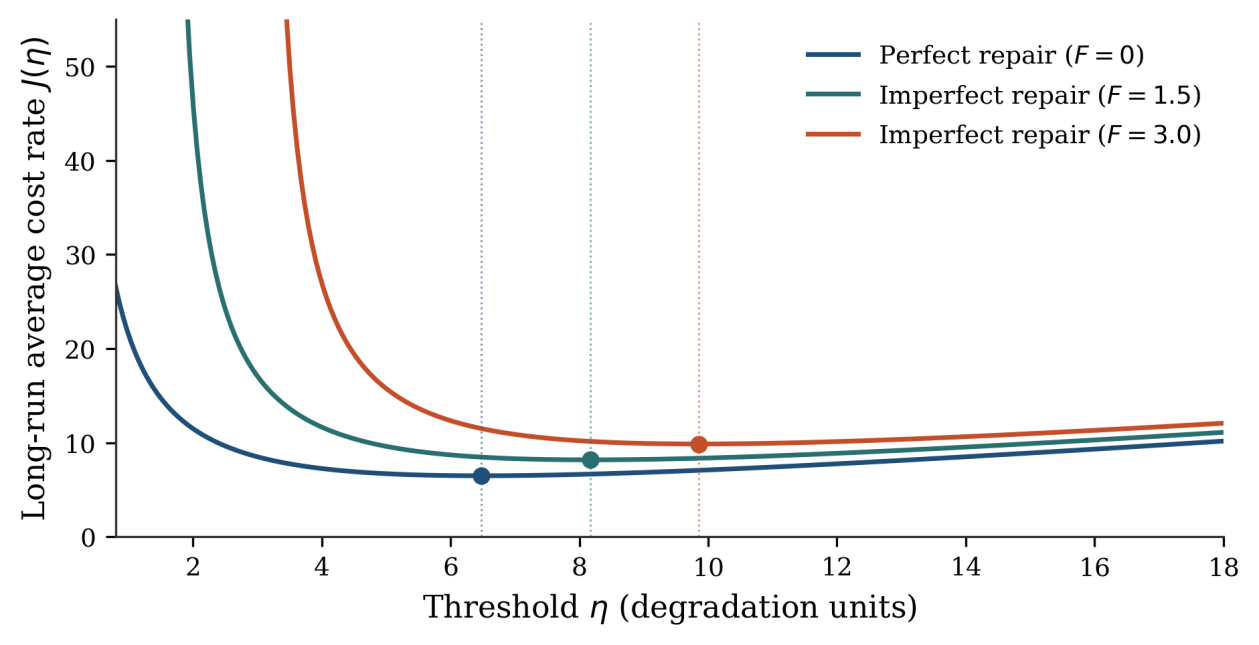
\includegraphics[width=\columnwidth]{figs/fig3_cost_curves.png}
\caption{Long-run average cost rate as a function of the degradation threshold, for perfect repair and two imperfect-repair levels. Dots mark the minimizers. Residual forgetting both raises the optimal cost rate and shifts the optimal threshold.}\label{fig:cost}
\end{figure}

\section{Multi-Action Scheduling as an Average-Cost MDP}\label{sec:mdp}
\subsection{State, Action, and Transition}
Time is discretized into decision epochs. The state is $x=(d,r)$, where $d$ is the discretized degradation index and $r$ is a coarse estimate of the current drift-hazard regime (for example, an indicator of whether the time since the last shock is in a decreasing- or increasing-mean-residual-life phase). The regime evolves as an exogenous Markov chain, independent of $d$ and of the action. At each epoch the maintainer chooses a parametric action
\begin{equation}
a\in\mathcal A=\{\text{no-op, knowledge edit, parameter-efficient fine-tune, full retrain}\},
\end{equation}
with cost $K(a)$, forgetting increment $F(a)$, and degradation-reduction fraction $\rho(a)\in[0,1]$, so that
\begin{equation}
d'=(1-\rho(a))\,d+F(a)+\zeta,
\label{eq:trans}
\end{equation}
where $\zeta$ is the random staleness increment accrued during the epoch, with a law that depends on $r$. Retrieval is deliberately not an element of $\mathcal A$. It does not reduce degradation already in $d$; it lowers the mean of $\zeta$ from $\gamma$ to $\gamma-\alpha$ per unit time at upkeep $k_C$. Whether to keep the store is an outer comparison of the optimal average costs with and without retrieval (Section~\ref{sec:rag}).

\subsection{Optimality Equation}
The one-step cost is $c(d,a)=c_L d+K(a)+c_F F(a)$. The average-cost optimality equation \cite{puterman1994,bertsekas2017} is
\begin{equation}
g+V(d,r)=\min_{a\in\mathcal A}\Big\{c(d,a)+\sum_{d',r'}P(d',r'\mid d,r,a)\,V(d',r')\Big\},
\label{eq:bellman}
\end{equation}
where $g$ is the optimal average cost rate and $V$ is a relative value function, unique up to an additive constant. The state space is low-dimensional by design, so \eqref{eq:bellman} is solvable by relative value iteration for any numerical instantiation. The point of this section is the structural property that survives across parameterizations.

\subsection{Control-Limit Theorem}
\begin{proposition}[Monotone control-limit policy]\label{prop:cl}
Suppose Assumption~\ref{as:monotone} holds. Then $V(\cdot,r)$ is nondecreasing in $d$ for each regime $r$, and there exists an average-cost optimal policy $\pi^\ast$ that is nondecreasing in $d$: there are thresholds $0\le\eta_1(r)\le\eta_2(r)\le\eta_3(r)$ such that the optimal action escalates through the ordered set \{no-op, edit, efficient fine-tune, full retrain\} as $d$ crosses each threshold in turn.
\end{proposition}
The argument is standard and is given in the Appendix. One first establishes monotonicity and submodularity of the discounted value iterates by preservation of increasing tails and by Topkis's theorem \cite{topkis1998}, and then passes to the average-cost limit along a sequence of discount factors under the unichain assumption \cite{puterman1994}.

Two remarks delimit the result. Condition (i) holds automatically for the transition \eqref{eq:trans} because a larger $d$ shifts $d'$ upward by the factor $(1-\rho(a))$. Condition (iii) is not automatic: it depends on the tail shape of $\zeta$ and on the forgetting increments. It holds without further conditions for replacement-type actions with $\rho=1$, because the next state then does not depend on $d$ while the no-action next state is stochastically increasing in $d$. In general it can be checked on the discretized kernel. Convexity of $V$ is neither claimed nor needed.

The single-threshold policy of Section~\ref{sec:shock} is the special case $|\mathcal A|=2$ with $F=0$. Proposition~\ref{prop:cl} is the multi-action analogue of the control-limit policies that are optimal for monotone degradation processes \cite{wang2002}. It gives formal support to an escalation already used informally in operations pipelines (edit, then efficient fine-tune, then full retrain, with a retrieval store as a separate input) as the optimal qualitative shape under stated conditions, not as an engineering convenience.

The thresholds depend on the regime $r$, but the proposition does not sign that dependence. The closed form \eqref{eq:sqrt} shows why intuition can mislead: higher drift intensity raises $\eta^\ast$ and shortens $t^\ast$. In a high-hazard regime the policy maintains more often in calendar time, though not necessarily at a lower degradation level. The direction for a fitted model is a numerical output of relative value iteration.

\subsection{Computation and a Caveat}
Relative value iteration fixes a reference state, initializes $V=0$, and iterates the Poisson-equation form of \eqref{eq:bellman} until the differential value and the subtracted reference term, which converges to $g$, stabilize; an aperiodicity transformation is applied if needed. Because the state space is a scalar degradation grid crossed with a handful of regimes, the computation is cheap relative to a single knowledge edit on a deployed model and can be re-solved as drift parameters are re-estimated. If Assumption~\ref{as:monotone} fails, the algorithm remains valid and simply returns whatever policy is optimal, so it doubles as a diagnostic for violations.

The principal caveat is that $F$ is taken to depend on the action only. If an aggressive fine-tune from an already very stale state induces disproportionately severe forgetting, because the optimizer must travel further so that $F=F(a,d)$, then both the increasing-tail and the submodularity conditions can fail, and the optimal policy need not be monotone. Section~\ref{sec:imperfect} suggests this is possible whenever the required displacement direction rotates as staleness accumulates. A non-monotone numerical policy is then a prediction of the model and not a defect of the solver.

\section{Retrieval as a Feedback Compensator}\label{sec:rag}
\subsection{Effective Staleness}
Parametric actions displace $\theta$ and therefore incur $F$. Retrieval reduces observed staleness by conditioning generation on passages from a corpus $C(t)$ that can be refreshed independently. In the notation of Section~\ref{sec:model}, a working retrieval system replaces $A(\theta,W)$ by an augmented functional $A(\theta,W,C)$, and the effective staleness is
\begin{equation}
S_{\mathrm{eff}}(t)=S(t)-R(t),
\end{equation}
where $R(t)$ is the reduction attributable to retrieval. It increases with the recency and coverage of $C$ relative to $W$ and is bounded above by retrievability: a new fact that can be indexed is absorbable, whereas a change in required reasoning style or safety norm is not.

\subsection{Blending Condition}
Suppose the store is kept current at upkeep $k_C$ per unit time and absorbs drift at average rate $\alpha$, so that effective staleness grows at $\gamma-\alpha$ between parametric events. Substituting $\gamma-\alpha$ for $\gamma$ in Section~\ref{sec:shock} gives
\begin{equation}
\eta_C^\ast=\sqrt{\frac{2K_R(\gamma-\alpha)}{c_L}},\qquad t_C^\ast=\sqrt{\frac{2K_R}{c_L(\gamma-\alpha)}}.
\label{eq:retr}
\end{equation}
Relative to the no-retrieval optimum, the store lowers the staleness threshold by the factor $\sqrt{1-\alpha/\gamma}$ and lengthens the parametric interval by the reciprocal factor $\sqrt{\gamma/(\gamma-\alpha)}$. Comparing average costs yields the investment test
\begin{equation}
k_C<J^\ast(\gamma)-J^\ast(\gamma-\alpha)=\sqrt{2K_Rc_L\gamma}\Big(1-\sqrt{1-\alpha/\gamma}\Big).
\label{eq:invest}
\end{equation}
Retrieval alone, with no parametric maintenance, is never optimal when $\gamma>\alpha$: effective staleness then grows without bound under the affine model and the average cost diverges. Blending therefore dominates both pure strategies exactly when \eqref{eq:invest} holds. The substitution is partial and bounded by $\alpha$. Forms of drift that retrieval cannot correct still accumulate at their full rate against the parametric model and must eventually be repaired by the mechanisms of Sections~\ref{sec:imperfect} and \ref{sec:mdp}. For the measured share $\alpha/\gamma\approx0.61$ of Section~\ref{sec:num}, the right-hand side of \eqref{eq:invest} is about $0.38\sqrt{2K_Rc_L\gamma}$, so the store is worth keeping whenever its upkeep is below roughly 38\% of the optimal no-retrieval cost rate.

\subsection{A Monitoring Caveat}
The reduction $R$ can be negative in effect when retrieved evidence is irrelevant or contradictory. For planning purposes $\alpha$ is therefore an empirically monitored slope, estimated by the regression of Section~\ref{sec:est} on a retrieval-on sample, not a design parameter that can be assumed correct once a store has been deployed.

\section{Numerical Results and Measurement Study}\label{sec:num}
\subsection{Purpose}
Sections~\ref{sec:num}-B and \ref{sec:num}-C illustrate the comparative statics with stylized parameters chosen for readability and not for calibration; only the ratios in Table~\ref{tab:sqrt} are meaningful. Section~\ref{sec:num}-D then instantiates the measured inputs on a public model.

\subsection{Square-Root Comparative Statics}
The single-threshold model is instantiated with leak $\beta=0.01$ staleness units per day, event rate $\lambda\in\{0.05,0.10,0.20,0.40\}$ per day, mean mark $\mu_\xi=1$, and operating-loss coefficient $c_L=1$. The retrain cost $K_R$ is swept over $\{10^2,10^4,10^6\}$ to stand for a small fine-tune, a mid-size continual-pretraining run, and a large full retrain. Table~\ref{tab:sqrt} reports $t^\ast$ and $J^\ast$ from \eqref{eq:sqrt}.

\begin{table*}[t]
\caption{Optimal Cycle Length $t^\ast$ (Days) and Cost Rate $J^\ast$ From the Square-Root Formula, With $\beta=0.01$, $\mu_\xi=1$, and $c_L=1$}\label{tab:sqrt}
\centering
\footnotesize
\begin{tabular}{cccccccc}
\toprule
$\lambda$ (per day) & $\gamma$ & $t^\ast$, $K_R\!=\!10^2$ & $t^\ast$, $K_R\!=\!10^4$ & $t^\ast$, $K_R\!=\!10^6$ & $J^\ast$, $K_R\!=\!10^2$ & $J^\ast$, $K_R\!=\!10^4$ & $J^\ast$, $K_R\!=\!10^6$\\
\midrule
0.05 & 0.06 & 57.7 & 577.4 & 5773.5 & 3.46 & 34.64 & 346.41\\
0.10 & 0.11 & 42.6 & 426.4 & 4264.0 & 4.69 & 46.90 & 469.04\\
0.20 & 0.21 & 30.9 & 308.6 & 3086.1 & 6.48 & 64.81 & 648.07\\
0.40 & 0.41 & 22.1 & 220.9 & 2208.6 & 9.06 & 90.55 & 905.54\\
\bottomrule
\end{tabular}
\end{table*}

Three patterns are worth stating. First, with $K_R$ fixed, $t^\ast$ falls by a factor of two when $\gamma$ rises fourfold: a fourfold acceleration of the world justifies only a halving of the interval. Across the grid, $\gamma$ rises by a factor of 6.8, so $t^\ast$ falls, and $\eta^\ast$ and $J^\ast$ rise, by a factor of $\sqrt{6.8}\approx2.6$ in every column. Second, moving from the smallest to the largest cost regime (a factor of $10^4$) lengthens $t^\ast$ by a factor of 100, again the square-root curvature. Third, the forgetting-augmented optimum of Section~\ref{sec:imperfect} implies that, at fixed $K$, a smaller $F$ lowers $J^\ast$ through both the one-off term and the permanent term, and it simultaneously shortens $t^\ast$. Investment in a less damaging repair technology therefore pays twice: directly, by lowering the damage per event, and indirectly, by making it economical to maintain more often. Fig.~\ref{fig:sqrt} plots the same relationships continuously in the drift intensity.

\begin{figure}[t]
\centering
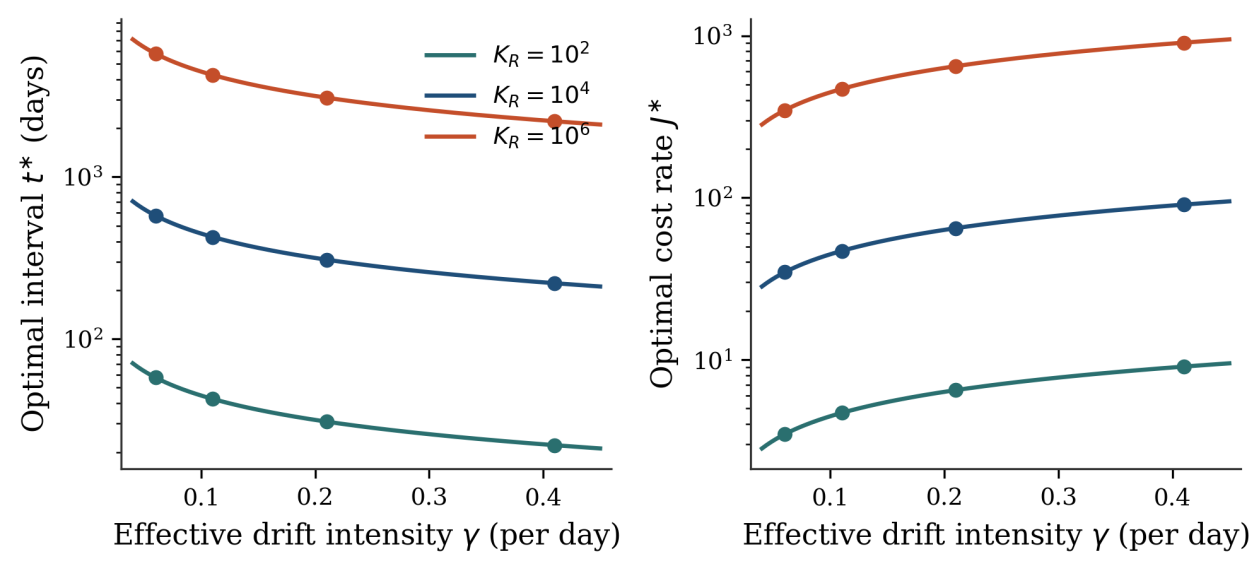
\includegraphics[width=\columnwidth]{figs/fig2_sqrt_statics.png}
\caption{Square-root comparative statics of the single-threshold program. Markers correspond to the grid in Table~\ref{tab:sqrt}. The optimal interval declines as the square root of drift intensity; the optimal cost rate increases as the square root of intensity and of retrain cost.}\label{fig:sqrt}
\end{figure}

\subsection{Hazard-Regime Sensitivity}
A Weibull inter-event law with shape above one gives an increasing hazard and a decreasing mean residual life; shape below one gives the opposite; shape one recovers the Poisson case. Section~\ref{sec:shock} predicts that a policy that shortens the calendar interval as time since the last shock grows beats the memoryless threshold under decreasing mean residual life, and that the same heuristic loses under increasing mean residual life. We have not run this experiment. For any fitted arrival model the predictions can be checked by solving the regime-dependent MDP of Section~\ref{sec:mdp}. If they are confirmed, the shape of the arrival hazard is a first-order determinant of the policy class an organization should adopt, and it is estimable from historical detector alarms.

\subsection{Measurement on a Public Pretrained Model}
The measurement side of the framework is instantiated on EleutherAI Pythia-70M \cite{biderman2023} with a synthetic world of facts that cannot occur in pre-training. The world has 150 fictional companies, each with three dynamic attributes (chief executive, headquarters city, main product; 450 facts) that are subject to drift, and one static attribute (founding year; 150 facts) that never changes and serves as the retention suite. Each attribute has eight candidate values. The model is scored as correct if the true value receives the highest summed token log-probability among the eight candidates given a fixed prompt. Staleness is the error rate on the dynamic suite in percentage points; forgetting is the change in error rate on the static suite, where one static fact equals 0.67 percentage points.

Drift events arrive as a Poisson process with rate three per day, each replacing one randomly chosen dynamic fact. Seventy percent of events are detected and logged. Sixty percent of the dynamic facts are indexed in an external store refreshed daily. The deployed checkpoint at $t=0$ is obtained by fine-tuning the pretrained model until it answers at least 95\% of the dynamic suite, the static suite, and the dynamic suite with retrieved notes correctly. The training mix includes notes that conflict with the memorized value, so that the model learns to follow retrieved text; this took 65 to 175 epochs depending on the seed. Every number below is a mean over ten random seeds. Each seed draws its own company names and facts, drift stream, indexed subset, and deployed checkpoint. Intervals are 95\% $t$-intervals across seeds.

Three parametric repairs are applied, separately and from the same deployed checkpoint, after 10 and 30 days of drift. The localized edit updates the MLP block of one layer on the logged facts whose value has changed, together with ten unchanged facts per edited fact; the replayed facts act as a locality constraint. The LoRA adapter \cite{hu2022} has rank 16 on all layers and no replay. The full fine-tune updates all parameters on the current value of every fact. Learning rates and epoch counts were fixed on a separate pilot seed that is not among the ten reported. For each mechanism we took the setting with the fewest processed tokens whose accuracy on the facts it was trained on was at least 0.9 and, for the edit, whose accuracy on untouched facts was at least 0.95. This rule was written down before the final pilot round and uses neither total error nor retention. The pilot results are part of the supplementary material.

Over 60 days without parametric maintenance, OLS yields a slope of 0.525 percentage points per day without retrieval (95\% CI 0.503 to 0.547; mean $R^2=0.99$) and 0.213 with a daily retrieval refresh (0.190 to 0.237; mean $R^2=0.98$). Both trajectories are well described by the affine mean of Section~\ref{sec:shock}. Over this horizon 180 events are expected, and the expected fraction of distinct dynamic facts that have changed at least once is $1-e^{-180/450}\approx0.33$ rather than one, so the affine fit is still a local approximation to a saturating process. Retrieval removes a share $1-0.213/0.525$ of the drift slope, which averages 0.593 across seeds (95\% CI 0.547 to 0.638). The indexed share of 0.60 lies inside this interval (one-sample $t$-test against 0.60, $p=0.73$): retrieval absorbs the share of drift that it covers, and no more. Substituting the per-seed share into \eqref{eq:retr} predicts that the store lengthens the economically optimal parametric interval by a factor of 1.58 (1.49 to 1.67) and lowers the optimal staleness threshold to 0.64 (0.60 to 0.67) of its no-retrieval value. Fig.~\ref{fig:drift} plots the two measured trajectories.

\begin{figure}[t]
\centering
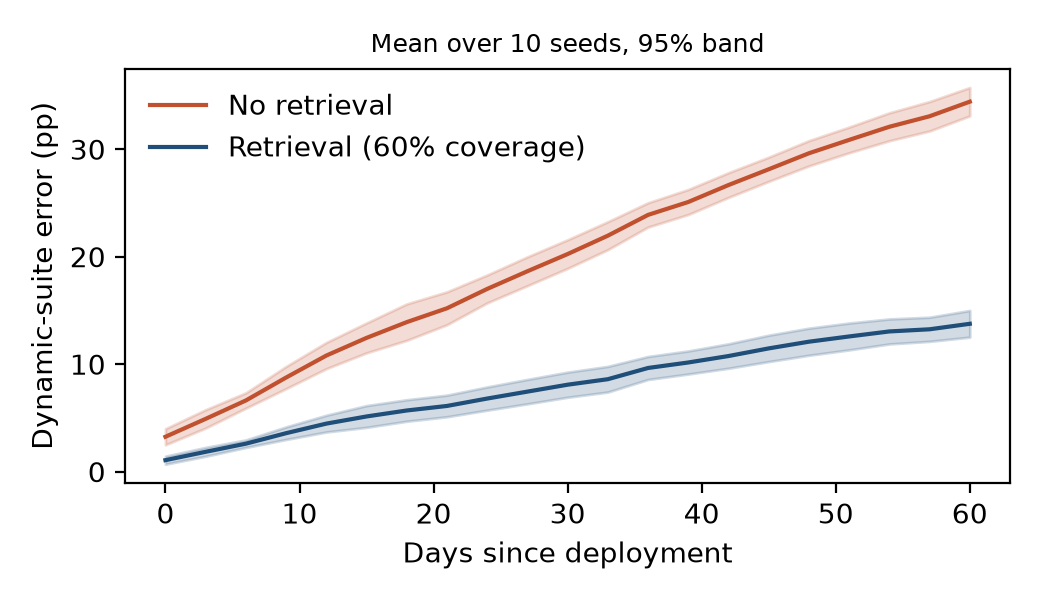
\includegraphics[width=\columnwidth]{figs/fig4_measured_drift.png}
\caption{Dynamic-suite error of the deployed Pythia-70M model over 60 days without parametric maintenance, scored every three days. Lines are means over ten seeds and bands are 95\% intervals across seeds. Retrieval over a corpus covering 60\% of the drifting facts reduces the fitted slope from 0.525 to 0.213 percentage points per day.}\label{fig:drift}
\end{figure}

\begin{table*}[t]
\caption{Measured Cost, Error Reduction, and Forgetting of Three Parametric Mechanisms on Pythia-70M (Ten Seeds)}\label{tab:mech}
\centering
\footnotesize
\begin{tabular}{llccccc}
\toprule
Mechanism & Trainable subset & Cost, $K'$ & Cost, $K$ & Error before $\to$ after (pp) & Retention change (pp) & Raises error (\%)\\
\midrule
Localized edit & MLP block of one layer & 37 & 636 & $16.7\to11.7$ & $-1.1$ (SD 1.5) & 40\\
LoRA, rank 16, no replay & Low-rank adapters, all layers & 1.4 & 71 & $16.7\to94.5$ & $+36.0$ (SD 11.6) & 100\\
Full fine-tune & All parameters & 1000 & 1000 & $16.7\to4.4$ & $-1.4$ (SD 1.8) & 5\\
\bottomrule
\end{tabular}\\[2pt]
\parbox{0.92\textwidth}{\footnotesize Means over ten seeds of the average of the interventions after 10 and 30 days of drift. Costs are normalized so that a full fine-tune equals 1000 units, under the trainable-parameter accounting $K'$ and the forward-inclusive accounting $K$ of Section~\ref{sec:model}. Error is the sum of dynamic-suite and static-suite error and can therefore exceed 100. Retention change is the change in static-suite error; one static fact is 0.67 pp. The last column is the share of the 20 interventions (ten seeds, two days) after which total error was not lower than before.}
\end{table*}

Table~\ref{tab:mech} gives the cost, error reduction, and forgetting of the three mechanisms. The full fine-tune is the most effective and by far the most expensive: it lowers total error by 12.3 pp (95\% CI 9.1 to 15.6) and raised it in only one of 20 interventions. The localized edit lowers total error by 5.1 pp (0.8 to 9.4) at a trainable-parameter cost 27 times smaller. Neither shows forgetting. Their retention changes of $-1.1$ and $-1.4$ pp are below two static facts and slightly negative, which is expected because the static facts are partly replayed. Fig.~\ref{fig:mech} summarizes the three columns of Table~\ref{tab:mech}.

\begin{figure}[t]
\centering
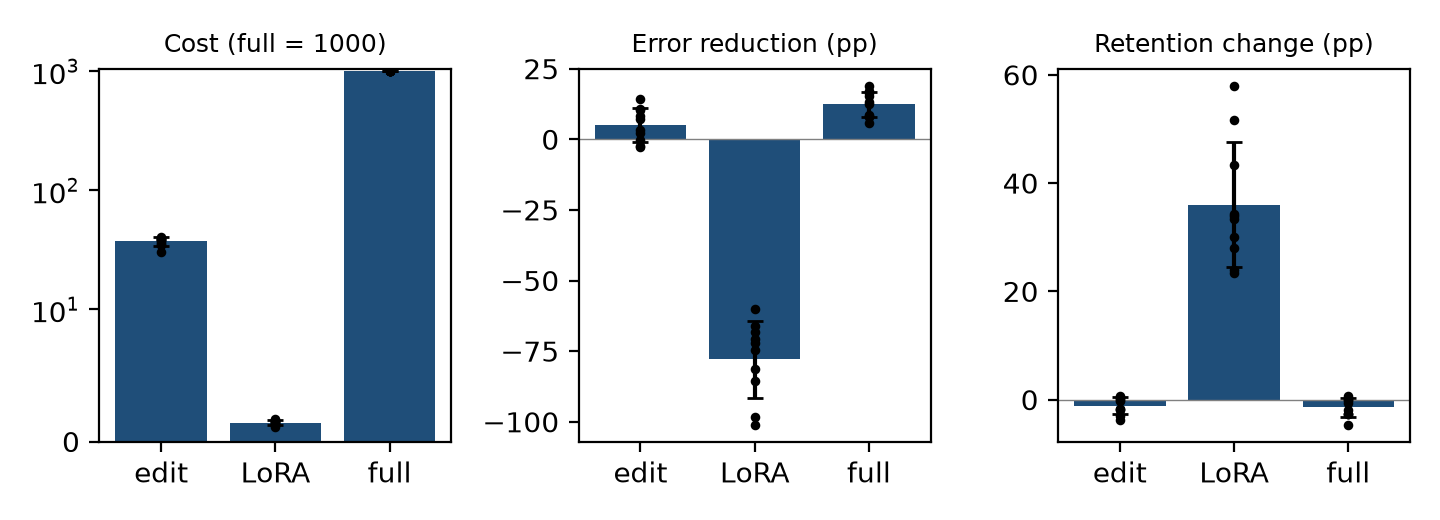
\includegraphics[width=\columnwidth]{figs/fig5_mechanisms.png}
\caption{Measured cost, error reduction, and forgetting of the three parametric mechanisms in Table~\ref{tab:mech}; bars are means over ten seeds with one standard deviation, dots are single seeds. The unreplayed low-rank adapter is cheap but raises total error and retention error, and is therefore dominated by taking no action.}\label{fig:mech}
\end{figure}

The benefit of the edit depends on the state in which it is applied. After 10 days, when total error before repair averages 11.4 pp, the edit changed total error by $+0.9$ pp on average and raised it in six of ten seeds. After 30 days, at 22.0 pp, it lowered error by 11.1 pp and raised it in two of ten seeds. This is the pattern a control-limit policy exploits, doing nothing below a threshold and editing above it. Two maintenance epochs are too few to estimate the threshold, so we offer this as an observation and not as a test of Proposition~\ref{prop:cl}. Two qualifications apply. First, the edit worked only with locality replay. In a pilot with one replayed fact per edited fact, the edit settings that fitted at least 0.9 of the edited facts still raised total error by 22 to 34 pp, because the update overwrote unchanged dynamic facts. Second, the fixed settings did not transfer evenly across seeds. The mean accuracy on the facts being repaired was 0.65 for the edit (0.15 to 1.00 across seeds) and 0.85 for the full fine-tune, against 0.95 and 0.99 on the pilot seed. We did not investigate the cause.

The edit's cost advantage also depends on the accounting. Under the trainable-parameter accounting, the edit removes about eleven times more error per cost unit than the full fine-tune (0.135 versus 0.012 pp per unit). Under the forward-inclusive accounting, which also charges a forward pass through all parameters and a backward pass down to the edited layer, the edit costs 636 against 1000 and the ranking reverses (0.0079 versus 0.0123). Part of the difference is the replay: the edit processes more tokens than the full fine-tune (about 73,000 against 58,000). In all ten seeds, the full fine-tune was both more effective and more expensive than the edit under the trainable-parameter accounting, so the order assumed in condition (ii) of Assumption~\ref{as:monotone} holds for these two actions.

The low-rank adapter does not follow the pattern. It is the cheapest of the three under both accountings, yet it raised total error from 16.7 to 94.5 pp, in every one of the 20 interventions, and raised static-suite error by 36.0 pp (SD 11.6). Accuracy on untouched facts fell to 46\%, against about 95\% after the edit and 98\% after the full fine-tune. An unreplayed adapter trained at a comparatively high learning rate on drifting facts alone produces a displacement that need not be orthogonal to high-curvature directions of the pre-update loss, which is consistent with this damage. Low rank bounds the Euclidean size of $\Delta\theta$ and does not by itself constrain the Fisher-weighted norm: parameter efficiency is not low forgetting. The result is not confined to one learning rate. In the pilot, no setting between $10^{-4}$ and $2\times10^{-3}$ lowered total error at either maintenance day.

The measured costs also break the nominal order of the action set, because the efficient action is cheaper than the edit instead of more expensive. The adapter is nevertheless harmless to the policy. It costs more than no action, forgets more, and leaves a higher next-state error, so it is dominated. Because $V$ is nondecreasing in $d$, an action whose one-step cost is higher and whose next state is stochastically larger than those of no action is never strictly preferred. Removing it leaves the ordered set \{no-op, localized edit, full fine-tune\}. We report the configuration as measured instead of tuning it away because it shows that the ordering in Proposition~\ref{prop:cl} is a property to be verified from a table of the form of Table~\ref{tab:mech}.

The study validates the framework at the level of its inputs, on a small model with synthetic drift, replicated over ten seeds. Validation at the level of the scheduling decision itself, namely a closed-loop comparison of a periodic calendar with the control-limit policy of Proposition~\ref{prop:cl}, and replication on larger models, is left open.

\subsection{Summary of Findings}
Six findings close the analysis. (1) Under Poisson arrivals the optimal interval grows with the square root of retrain cost and shrinks with the square root of drift intensity, while the tolerated staleness grows with both. (2) The adequacy of a memoryless threshold is hypothesized to depend on the ageing property of the arrival law, with opposite prescriptions for a long quiet interval. (3) Forgetting is a Fisher-weighted quadratic form; lower forgetting per event lowers the optimal cost rate and shortens the optimal interval. (4) Under Assumption~\ref{as:monotone}, an optimal policy over a graduated menu is a nested control-limit rule. (5) Retrieval lengthens the parametric interval by $\sqrt{\gamma/(\gamma-\alpha)}$, dominates parametric maintenance alone when \eqref{eq:invest} holds, and cannot substitute when drift is not retrievable. (6) On Pythia-70M over ten seeds, measured staleness grows affinely with a retrieval share equal to coverage (0.59 against 0.60), full fine-tuning is the most effective repair, a localized edit helps on average but only with a locality constraint and not at low staleness, and an unreplayed low-rank adapter is dominated by no action in every intervention.

\section{Discussion}\label{sec:disc}
\subsection{Limitations and Further Work}
\emph{Identifiability.} The estimator of Section~\ref{sec:est} needs repeated full cycles: staleness accumulating from a reset, a repair, and a subsequent reset. Organizations that repair very infrequently, or that change mechanism or scoring method between cycles, may lack the record needed to estimate $\gamma$, let alone the hazard structure. In that data-poor regime the qualitative square-root sensitivities are more useful than a point estimate of $\eta^\ast$.

\emph{Scalar accuracy.} Assumption~\ref{as:scalar} collapses many task axes into one index. A vector-valued extension, with per-cluster staleness and selective actions of the kind knowledge editing already implements, would connect the model to multi-component maintenance with economic dependence \cite{dekker1997} and would test the robustness of Proposition~\ref{prop:cl} under a genuinely multi-objective cost.

\emph{Endogenous world.} Assumption~\ref{as:exo} is already strained by the presence of model-generated text in subsequent training corpora. Letting the arrival rate $\lambda$ depend on cumulative prior deployment would link the renewal program to the literature on degradation induced by training on model-generated data \cite{shumailov2024}.

\emph{Nonstationary primitives.} If $\beta$, $\lambda$, and $\mu_\xi$ themselves drift, the fixed-parameter control problem becomes an adaptive-control problem, and the estimator of Section~\ref{sec:est} must be replaced by an online filter.

\emph{Empirical scope.} The measurement study is a controlled experiment on one 70-million-parameter checkpoint with synthetic drift, ten seeds, two maintenance epochs per seed, and a closed eight-way scoring rule. It confirms the model's inputs but not the scheduling result on a production horizon. Repair settings were fixed on one pilot seed and fitted the repaired facts unevenly on the reported seeds, and the localized edit includes a replay constraint that is a design choice. The cost comparison also depends on which floating-point accounting is used, and the edit's cost advantage over full fine-tuning largely disappears under the forward-inclusive accounting. The natural next step is to fit $(\gamma,\alpha,K(a),F(a),\rho(a))$ on telemetry from a deployed system and to compare the control-limit policy with the incumbent calendar in closed loop.

\subsection{Operational Implications}
Four rules survive these limitations and do not require a precisely fitted $\eta^\ast$. First, set the cadence from measured $\gamma$ and $K_R$ through the square-root formula; a tenfold rise in update cost justifies only about a threefold longer interval, and a fourfold rise in drift intensity justifies a halved interval, not a quartered one. Second, admit a mechanism to the menu only after measuring its cost, its error reduction, its forgetting on a fixed retention suite, and, for edits, its effect on untouched facts, in the format of Table~\ref{tab:mech}; a name such as low-rank adaptation does not guarantee a place in the order. Third, treat the forgetting tolerance $\eps$ and the unit cost $c_F$ as governance parameters rather than trainer hyperparameters; residual forgetting imposes a permanent flow that no cadence removes, so a cheap damaging repair can lose to an expensive safe one. Fourth, invest in retrieval when \eqref{eq:invest} holds and only for the share of drift the corpus actually covers; that coverage is an operational metric to be re-estimated, not a one-time design choice.

\section{Summary and Conclusions}\label{sec:concl}
Maintaining a deployed LLM, that is, deciding when, how much, and by which mechanism to update it, is a CBM problem for a deteriorating system whose repair technology can itself damage the plant. Modeling staleness as a shock-and-wear process, forgetting as a Fisher-weighted imperfect repair, and mechanism selection as an average-cost MDP yields closed forms in restricted cases and a structural theorem for the graduated menu. The square-root law ties update cost and drift intensity to the economically optimal interval. The imperfect-repair comparative static says that safer repairs should be used more often. Retrieval is a compensator that substitutes only for the absorbable share of drift, and a closed-form test says when it is worth its upkeep. A small-model measurement study, replicated over ten seeds, confirms the affine and coverage assumptions and shows that the monotone action order is a measured property of mechanisms, not an article of faith: the localized edit pays off only with a locality constraint and at sufficient staleness, and an unreplayed low-rank adapter is dominated by no action.

The central claim is methodological. Treating language-model upkeep as a stochastic control problem, instead of as separately tuned heuristics for drift detection, forgetting mitigation, and cost control, explains patterns already visible in cadence studies and produces falsifiable predictions that can be taken to production telemetry.

\appendices
\section{Proof of Proposition~\ref{prop:cl}}
Consider first the $\alpha$-discounted problem with value iterates $V^{\alpha}_{n+1}(d,r)=\min_a\{c(d,a)+\alpha\,\E[V^{\alpha}_n(d',r')\mid d,r,a]\}$ and $V^{\alpha}_0\equiv0$, where $\alpha\in(0,1)$ denotes the discount factor in this appendix only. Suppose $V^{\alpha}_n$ is nondecreasing in $d$ for every $r$. Because the regime evolves independently of $(d,a)$, the expectation at fixed $r'$ is a nonnegative combination of tail probabilities of $d'$. By Assumption~\ref{as:monotone}(i) those tails are nondecreasing in $d$, so the expectation is nondecreasing in $d$. The one-step cost is nondecreasing in $d$, hence so is $V^{\alpha}_{n+1}$. By induction every iterate is nondecreasing, and so is the discounted limit $V^{\alpha}$.

For submodularity, Assumption~\ref{as:monotone}(iii) states that $\E[V(d',r')\mid d,r,a]$ is submodular in $(d,a)$ whenever $V$ is nondecreasing. The one-step cost is separable in $(d,a)$ and therefore modular. The Bellman operator thus preserves submodularity in $(d,a)$, and Topkis's monotonicity theorem implies that the largest minimizer of the right-hand side is nondecreasing in $d$. This holds for every discounted problem. There are finitely many deterministic stationary policies, so some monotone policy is discount-optimal along a sequence $\alpha_k\to1$. Under the unichain assumption that policy is average-cost optimal, and $V$ inherits monotonicity from $V^{\alpha}$ \cite[Ch.~8]{puterman1994}. A monotone map from a totally ordered state coordinate to a totally ordered finite action set is characterized by the nested thresholds stated in the proposition.

Condition (i) holds for \eqref{eq:trans} because $d'=(1-\rho(a))d+F(a)+\zeta$ is increasing in $d$ for each fixed $(a,\zeta)$. For replacement actions with $\rho(a)=1$, $d'$ does not depend on $d$ while the no-action transition is stochastically increasing in $d$, so the difference of expected continuations is nonincreasing in $d$ and Assumption~\ref{as:monotone}(iii) holds for those pairs without further restrictions. \hfill$\blacksquare$

\section{Notation}
\begin{table}[h]
\caption{Principal Symbols}\label{tab:notation}
\centering
\footnotesize
\begin{tabular}{p{0.28\columnwidth}p{0.62\columnwidth}}
\toprule
Symbol & Meaning\\
\midrule
$\theta(t),\ \Delta\theta$ & Parameter vector; displacement at a maintenance event\\
$W(t),\ C(t)$ & World state; external retrieval corpus\\
$A,\ S,\ F,\ D$ & Freshness; staleness; forgetting; degradation index $S+F$\\
$K,\ \kappa,\ k_C$ & Action cost; operations-to-money factor; retrieval upkeep rate\\
$c_L,\ c_F$ & Loss rate on degradation; one-off cost per unit of forgetting\\
$(T_i,\xi_i),\ \lambda,\ \mu_\xi,\ \beta,\ \gamma$ & Drift epochs and marks; Poisson rate; mean mark; leak; $\gamma=\beta+\lambda\mu_\xi$\\
$m(t),\ \eta,\ t(\eta)$ & Renewal function; degradation threshold; cycle length\\
$I(\theta),\ \eps$ & Diagonal Fisher matrix on the old world; forgetting tolerance\\
$\pi,\ \rho(a),\ \zeta$ & Plasticity; degradation-reduction fraction; epoch increment\\
$(d,r),\ \mathcal A,\ g,\ V$ & MDP state; action set; average cost; relative value\\
$R,\ \alpha,\ S_{\mathrm{eff}}$ & Retrieval reduction; absorbed drift rate; effective staleness\\
\bottomrule
\end{tabular}
\end{table}

\section*{Acknowledgment}
This research did not receive any specific grant from funding agencies in the public, commercial, or not-for-profit sectors.

\section*{CRediT Authorship Contribution Statement}
Ook Lee: Conceptualization, Methodology, Formal analysis, Investigation, Writing -- original draft, Writing -- review and editing.

\section*{Declaration of Competing Interest}
The author declares that he has no known competing financial interests or personal relationships that could have appeared to influence the work reported in this paper.

\section*{Data Availability}
The measurement study uses the public EleutherAI Pythia-70M checkpoint. The code that generates the synthetic world and runs the training, drift simulation, and scoring, the per-seed result files for all ten reported seeds, and the pilot results used to fix the repair settings will be deposited in a public archive, and the DOI will be inserted before publication. No proprietary organizational telemetry is used.

\begin{thebibliography}{99}
\bibitem{arts2025} J. Arts, R. N. Boute, S. Loeys, and H. E. van Staden, ``Fifty years of maintenance optimization: Reflections and perspectives,'' \emph{Eur. J. Oper. Res.}, vol. 322, no. 3, pp. 725--739, 2025.
\bibitem{barlow1965} R. E. Barlow and F. Proschan, \emph{Mathematical Theory of Reliability}. New York, NY, USA: Wiley, 1965.
\bibitem{bertsekas2017} D. P. Bertsekas, \emph{Dynamic Programming and Optimal Control}, 4th ed., vol. I. Belmont, MA, USA: Athena Scientific, 2017.
\bibitem{beytur2025} H. B. Beytur, G. de Veciana, H. Vikalo, and K. S. Chan, ``Optimal resource allocation for ML model training and deployment under concept drift,'' 2025, arXiv:2512.12816.
\bibitem{biderman2023} S. Biderman \emph{et al.}, ``Pythia: A suite for analyzing large language models across training and scaling,'' in \emph{Proc. 40th Int. Conf. Mach. Learn.}, 2023, pp. 2397--2430.
\bibitem{dejonge2020} B. de Jonge and P. A. Scarf, ``A review on maintenance optimization,'' \emph{Eur. J. Oper. Res.}, vol. 285, no. 3, pp. 805--824, 2020.
\bibitem{dekker1996} R. Dekker, ``Applications of maintenance optimization models: A review and analysis,'' \emph{Rel. Eng. Syst. Saf.}, vol. 51, no. 3, pp. 229--240, 1996.
\bibitem{dekker1997} R. Dekker, R. E. Wildeman, and F. A. van der Duyn Schouten, ``A review of multi-component maintenance models with economic dependence,'' \emph{Math. Methods Oper. Res.}, vol. 45, no. 3, pp. 411--435, 1997.
\bibitem{gao2023} Y. Gao \emph{et al.}, ``Retrieval-augmented generation for large language models: A survey,'' 2023, arXiv:2312.10997.
\bibitem{hoffmann2022} J. Hoffmann \emph{et al.}, ``Training compute-optimal large language models,'' 2022, arXiv:2203.15556.
\bibitem{hu2022} E. J. Hu \emph{et al.}, ``LoRA: Low-rank adaptation of large language models,'' in \emph{Proc. Int. Conf. Learn. Represent.}, 2022.
\bibitem{huszar2018} F. Huszár, ``Note on the quadratic penalties in elastic weight consolidation,'' \emph{Proc. Natl. Acad. Sci. U.S.A.}, vol. 115, no. 11, pp. E2496--E2497, 2018.
\bibitem{jardine2006} A. K. S. Jardine, D. Lin, and D. Banjevic, ``A review on machinery diagnostics and prognostics implementing condition-based maintenance,'' \emph{Mech. Syst. Signal Process.}, vol. 20, no. 7, pp. 1483--1510, 2006.
\bibitem{kaplan2020} J. Kaplan \emph{et al.}, ``Scaling laws for neural language models,'' 2020, arXiv:2001.08361.
\bibitem{kirkpatrick2017} J. Kirkpatrick \emph{et al.}, ``Overcoming catastrophic forgetting in neural networks,'' \emph{Proc. Natl. Acad. Sci. U.S.A.}, vol. 114, no. 13, pp. 3521--3526, 2017.
\bibitem{kunstner2019} F. Kunstner, L. Balles, and P. Hennig, ``Limitations of the empirical Fisher approximation for natural gradient descent,'' in \emph{Adv. Neural Inf. Process. Syst.}, vol. 32, 2019.
\bibitem{lu2019} J. Lu, A. Liu, F. Dong, F. Gu, J. Gama, and G. Zhang, ``Learning under concept drift: A review,'' \emph{IEEE Trans. Knowl. Data Eng.}, vol. 31, no. 12, pp. 2346--2363, Dec. 2019.
\bibitem{luo2023} Y. Luo, Z. Yang, F. Meng, Y. Li, J. Zhou, and Y. Zhang, ``An empirical study of catastrophic forgetting in large language models during continual fine-tuning,'' 2023, arXiv:2308.08747.
\bibitem{mahadevan2023} A. Mahadevan and M. Mathioudakis, ``Cost-effective retraining of machine learning models,'' 2023, arXiv:2310.04216.
\bibitem{ouyang2022} L. Ouyang \emph{et al.}, ``Training language models to follow instructions with human feedback,'' in \emph{Adv. Neural Inf. Process. Syst.}, vol. 35, 2022.
\bibitem{pham1996} H. Pham and H. Wang, ``Imperfect maintenance,'' \emph{Eur. J. Oper. Res.}, vol. 94, no. 3, pp. 425--438, 1996.
\bibitem{puterman1994} M. L. Puterman, \emph{Markov Decision Processes: Discrete Stochastic Dynamic Programming}. New York, NY, USA: Wiley, 1994.
\bibitem{ross1996} S. M. Ross, \emph{Stochastic Processes}, 2nd ed. New York, NY, USA: Wiley, 1996.
\bibitem{shi2024} H. Shi \emph{et al.}, ``Continual learning of large language models: A comprehensive survey,'' 2024, arXiv:2404.16789.
\bibitem{shumailov2024} I. Shumailov, Z. Shumaylov, Y. Zhao, N. Papernot, R. Anderson, and Y. Gal, ``AI models collapse when trained on recursively generated data,'' \emph{Nature}, vol. 631, pp. 755--759, 2024.
\bibitem{topkis1998} D. M. Topkis, \emph{Supermodularity and Complementarity}. Princeton, NJ, USA: Princeton Univ. Press, 1998.
\bibitem{vannoortwijk2009} J. M. van Noortwijk, ``A survey of the application of gamma processes in maintenance,'' \emph{Rel. Eng. Syst. Saf.}, vol. 94, no. 1, pp. 2--21, 2009.
\bibitem{wang2002} H. Wang, ``A survey of maintenance policies of deteriorating systems,'' \emph{Eur. J. Oper. Res.}, vol. 139, no. 3, pp. 469--489, 2002.
\bibitem{wang2024} S. Wang, Y. Zhu, H. Liu, Z. Zheng, C. Chen, and J. Li, ``Knowledge editing for large language models: A survey,'' \emph{ACM Comput. Surv.}, vol. 57, no. 3, 2024.
\bibitem{williams2026} E. Williams, T. Sinha, M. Lyttle, and Y. Kanagasingam, ``Optimising retraining frequency for a paediatric emergency department admission prediction model,'' \emph{Emerg. Med. Australas.}, vol. 38, no. 3, 2026.
\bibitem{zhang2024} N. Zhang \emph{et al.}, ``A comprehensive study of knowledge editing for large language models,'' 2024, arXiv:2401.01286.
\end{thebibliography}

% \begin{IEEEbiographynophoto}{Ook Lee}
% (Biography to be supplied by the author.)
% \end{IEEEbiographynophoto}

\end{document}
